\documentclass[a4paper,11pt]{article}
\usepackage{a4wide}
\usepackage{fullpage}
\usepackage[utf8x]{inputenc}

\usepackage[light,math]{anttor}
\usepackage[T1]{fontenc}

%\usepackage[slovene]{babel}
%\selectlanguage{slovene}
\usepackage[toc,page]{appendix}
\usepackage[pdftex]{graphicx} 

\usepackage{lmodern}
\usepackage{amsmath}
\usepackage{amssymb}
\usepackage{amsthm}
\usepackage{amsfonts}
\usepackage{mathtools}
\usepackage{enumitem}
\usepackage{amsfonts}
\usepackage{amsmath}
\usepackage{setspace}
\usepackage{color}
\definecolor{light-gray}{gray}{0.95}
\usepackage{listings} 
\usepackage{hyperref}

\renewcommand{\baselinestretch}{1.2} 
\renewcommand{\appendixpagename}{Priloge}


\title{Algoritmi \\
\textbf{Domača naloga 1} }
\author{Sara Bizjak  |  27202020}
\date{Marec 2021}

%%%%%%%%%%%%%%%%%%%%%%%%%%%%%%%%%%%%%%%%%%%%%%%%%%%%%%%%%%%%%%%%%%%%%%%%%%%%%%%%%%%%%%%%%%%%%%%%%%%%%%%%%%%%%%%%%%%%%%%%%%%%%%%%%

\begin{document}

\maketitle

%%%%%%%%%%%%%%%%%%%%%%%%%%%%%%%%%%%%%%%%%%%%%%%%%%%%%%%%%%%%%%%%%%%%%%%%%%%%%%%%%%%%%%

\section*{Problem 1 -- Turingov stroj}

Sestavimo TS za množenje dveh števil, ki sta na traku podani v eniškem zapisu. 
\\
Poglejmo si primer množenja števil 3 in 4, kot je podan v navodilih naloge. 
Trak \textit{inputa} v tem primeru bi izgledal 
$$
B \ B \ 1 \ 1 \ 1 \ 0 \ 1 \ 1 \ 1 \ 1 \ 0 \ B \ B \ B \ B \ B \ \ldots
$$
kjer prve tri enke predstavljajo število 3, druge štiri pa število 4.
Ideja je, da za vsako enko izmed prvih treh, druge štiri enke kopiramo naprej na trak, kjer so sedaj zapisani $B$-ji oziroma prazni prostori.
Rezultat tega kopiranja bodo tako $3 \cdot 4 = 12$ enke, kar je ravno rezultat množenja med tema dvema številoma.
$$
B \ B \ B \ B \ B \ B \ B \ B \ B \ B \ B \ 1 \ 1 \ 1 \ 1 \ 1 \ 1 \ 1 \ 1 \ 1 \ 1 \ 1 \ 1 \ 0 \ B \ B \ B \ \ldots
$$
\noindent
Turingov stroj za množenje dveh eniško podanih števil predstavimo s sedmerko
$$
\left< \Sigma, Q, q_0, F, \delta, \Gamma, B \right>,
$$
kjer
\begin{align*}
\Sigma &= \{0, 1 \}
\\
Q &= \{ q_0, q_1, \ldots, q_8 \}
\\
q_0 &= \text{začetno stanje}
\\
F &= \text{končno stanje} = q_8
\\
\delta &= \{ 0, 1, B, Y \}
\\
\Gamma &= \text{prehodna funkcija (definirana v kodi)}
\\
\end{align*}
TS je bil konstruiran in opisan s pomočjo spletne strani \cite{bib:TS}.
Koda za poganjanje TS-ja na tej strani:
\\
\begin{lstlisting}
________________________________________________________________________
//-------CONFIGURATION
name: TS za mnozenje dveh enisko podanih stevil
init: q0
accept: q8
\end{lstlisting}
\begin{lstlisting}
//-------DELTA FUNCTION: 
\end{lstlisting}
\begin{minipage}{0.5\textwidth}
\begin{lstlisting}
q0,1
q1,_,>

q1,1
q1,1,>

q1,0
q2,0,>

q2,1
q3,Y,>

q3,1
q3,1,>

q3,0
q3,0,>

q3,_
q4,1,<

q4,1
q4,1,<

q4,0
q4,0,<

q4,Y
q2,Y,>
\end{lstlisting}
\end{minipage}\hfill
\begin{minipage}{0.5\textwidth}
\begin{lstlisting}
q2,0
q5,0,<

q5,Y
q5,1,<

q5,0
q5,0,<

q5,1
q5,1,<

q5,_
q0,_,>

q0,0
q6,_,>

q6,1
q6,_,>

q6,0
q7,_,>

q7,1
q7,1,>

q7,_
q8,0,>
\end{lstlisting}
\end{minipage}\hfill
\begin{lstlisting}
________________________________________________________________________
\end{lstlisting}

\newpage
\noindent
Pripadajoč tranzicijski graf:
\begin{figure}[ht!]
    \centering
    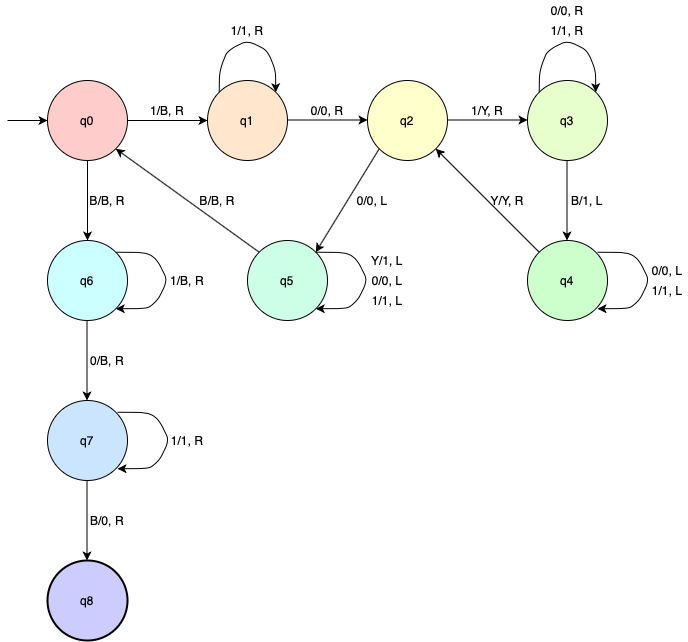
\includegraphics[width=150mm]{graf.png}
    \caption{Graf tranzicij stanj TS za množenje dveh eniško podanih števil.}
\end{figure}

\section*{Problem 2 -- Prevedba}
Pokažimo, da je problem delitve (\textit{partition problem}) NP-poln s prevedbo na problem seštevka podmnožic (\textit{subset-sum}). 
Cilj problema delitve je, da multi-množico pozitivnih celih števil $S$ razdelimo na dve podmnožici tako, da bosta vsoti elementov enaki.
Označimo ti dve podmnožici s $S_1$ in $S_2 = S - S_1$, kjer je $N_1$ vsota elementov iz $S_1$, $N_2$ pa vsota elementov iz $S_2$, tako da
$$
\sum_{s \ \in \ S_1} s = \sum_{s \ \in \ S_2} s 
$$
$$
\Rightarrow N_1 = N_2
$$
Ker je NP-poln problem hkrati NP in NP-težek problem, je za NP-polnost problema $L$ potrebno dokazati dvoje:
\begin{enumerate}
    \item Problem $L$ je vsebovan v razredu NP.
    \item Vsak drug (znan) problem $L'$ iz razreda NP lahko v polinomskem času prevedemo na problem $L$. 
\end{enumerate}
\noindent
Če problem ustreza drugemu pogoju, pravimo, da je problem NP-težek.
\\
\\
\textit{Dokaz vsebovanosti problema delitve v razredu NP.}
\\
Za primer delitve je certifikat particija na  $S_1$ in $S_2$. 
Očitno je, da lahko vsote obeh podmnožic preverimo v polinomskem (linearnem) času po naslednjem postopku:
\begin{enumerate}
    \item Preverimo, da z elementi iz $S_1$ in $S_2$ pokrijemo celoten $S$.
    \item Nastavimo $N_1 = 0$ in $N_2 = 0$.
    \item Za vsak element $s$ iz $S_1$ prištejemo njegovo vrednost $N_1$.
    \item Za vsak element $s$ iz $S_2$ prištejemo njegovo vrednost $N_2$.
    \item Preverimo, da sta vrednost $N_1$ in $N_2$ enaki.
\end{enumerate}
Ker lahko problem delitve rešimo v polinomskem času na nedetetminističnem TS, je torej vsebovan v razredu NP problemov.
\\
\\
\textit{Prevedba iz problema seštevka podmnožic na problem delitve.}
\\
Da bi pokazali, da je problem delitve NP-težek, reduciramo nek znan NP-poln problem, v našem primeru je to problem seštevka podmnožic, na problem delitve.
Pri reševanju problema seštevka podmnožic za \textit{input} vzamemo množico pozitivnih celih števil $S$ in končno, ciljno vsoto $t$. 
Poiskati moramo podmnožico $T \subset S$, katere vsota elementov je enaka $t$. 
Označimo z $N$ vsoto elementov iz $S$, torej $\sum_{s \in S} s = N$, in definirajmo množico 
$$S' = S \cup \{ N - 2t \},$$ 
ki jo podamo v problem delitve. 
Prevedba problema seštevka podmnožic na problem delitve očitno deluje v polinomskem času.
\\
\\
\textit{Dokaz, da ta prevedba res obstaja.}
\\
\textit{Predpostavimo, da ima problem seštevka podmnožic rešitev.}
\\
Denimo, da je $T$ množica števil z vsoto enako $t$. Tedaj imajo preostali elementi iz $S$, to množico označimo s $S_1$, vsoto $N_1 = N - t$. 
Nadalje, naj bo množica $S_2 = T \cup \{ N - 2t \}$ z vsoto $N_2$.
\\
Tedaj velja:
\begin{align*}
    N_1  &= N - t 
    \\
    N_1  - t &= N - 2t, 
\end{align*}
\noindent
kar nam podaja razliko med množicama $S_1$ in množico $T$.
\\
Nadalje velja:
\begin{align*}
    N_2 &= t + (N - 2t) 
\\
    &= N - t 
\\
    &= N_1,
\end{align*}
\noindent
kar pomeni, da sta vsoti elementov množic $S_2$ in $S_1$ enaki.
\\
Začetno množico $S$ lahko torej razdelimo na dve podmnožici, označili smo jih s $S_1$ in s $S_2$, katerih vsota elementov je pri obeh podmnožicah enaka $(N - t)$. 
\\
\textit{Obrat: Predpostavimo, da ima problem delitve rešitev.}
\\
Pokažimo še obratno in denimo, da v $S'$ obstajata dve podmnožici $S_1$ in $S_2$ z enakima vsotama $N - t$. Iščemo podmnožico $T$, ki ima vsoto enako $t$.
\\
$S'$ je definirana kot $S' = S \cup \{ N - 2t \}$, torej ena izmed $S_1$ in $S_2$ vsebuje $N - 2t$, BŠS je to $S_1$. Naj bo 
$$T = S_1 \setminus \{ N - 2t \}.$$
Vsota elementov iz $T$ je tedaj enaka 
$$N - t - (N - 2t) = t.$$ 
\\
Našli smo torej podmnožico $T$, ki zadošča problemu seštevka podmnožic.
\\
Dokazali smo, da ima problem seštevka podmnožic rešitev natako tedaj, ko ima problem delitve rešitev.
\\
\\
S tem smo dokazali NP-polnost problema delitve.

%%%%%%%%%%%%%%%%%%%%%%%%%%%%%%%%%%%%%%%%%%%%%%%%

\section*{Problem 3 -- Rodovne funkcije}
\subsection*{Problem 3.1.}
Izračunajmo na koliko načinov lahko dobimo vsoto $500$ evorov samo z bankovci po 10 in 20 evrov.
Z $G(z)$ označimo rodovno funkcijo, ki predstavlja zgoraj omenjene kombinacije -- zanimalo nas bo torej število $[z^{500}]G(z) = g_{500}$, kar je koeficient pri členu $z^{500}$. 
\\
Zapišimo rodovne funkcije za vsak relevanten bankovec posebej. Označimo z $R_{10}(z)$ rodovno funkcijo za bankovce po $10$ evrov in z $R_{20}(z)$ rodovno funkcijo za bankovce po $20$ evrov. Tedaj:
\begin{align*}
R_{10}(z) = 1 + z^{10} + z^{20} + z^{30} + z^{40} + \ldots = \sum_{n = 0}^{\infty} z^{10n}
\\
R_{20}(z) =  1 + z^{20} + z^{40} + z^{60} + z^{80} + \ldots = \sum_{n = 0}^{\infty} z^{20n}
\end{align*}
Rodovno funkcija za vse bankovce $G(z)$ zapišemo kot
\begin{align*}
    G(z) &= R_{10}(z) \cdot R_{20}(z) 
    \\
    &= \left( 1 + z^{10} + z^{20} + z^{30} + z^{40} + \ldots \right) \cdot \left( 1 + z^{20} + z^{40} + z^{60} + z^{80} + \ldots \right)
    \\
    &= \left( \sum_{n = 0}^{\infty} z^{10n} \right) \cdot \left( \sum_{n = 0}^{\infty} z^{20n} \right)
    \\
    &= \frac{1}{1 - z^{10}} \cdot \frac{1}{1 - z^{20}}   
\end{align*}
Hitro lahko seštejemo koeficiente pri členu $z^{500}$ in dobimo rezultat $g_{500} = 26$.
\\
\\
Sedaj poiščemo bolj jedrnato rodovno funkcijo, ki jo označimo z $G_c(z)$ in izpišemo $[z^{50}]G_c(z) = g_{c50}$.
Bolj kompaktno funkcijo vpeljemo zaradi operiranja z manjšimi potencami, 
glede na navodila naloge pa je njen pomen to, da je število načinov plačila $500$ evrov z bankovci po $10$ in $20$ evrov ekvivalent številu načinov plačila $50$ evorov s kovanci po $1$ in $2$ evra.
\\
Podobno kot pri $G(z)$ zapišemo tudi za $G_c(z)$:
\begin{align*}
    G_c(z) &= R_{1}(z) \cdot R_{2}(z) 
    \\
    &= \left( 1 + z^{1} + z^{2} + z^{3} + z^{4} + \ldots \right) \cdot \left( 1 + z^{2} + z^{4} + z^{6} + z^{8} + \ldots \right)
    \\
    &= \left( \sum_{n = 0}^{\infty} z^{n} \right) \cdot \left( \sum_{n = 0}^{\infty} z^{2n} \right)
    \\
    &= \frac{1}{1 - z} \cdot \frac{1}{1 - z^{2}}   
\end{align*}
Tudi tukaj hitro preštejemo koeficiente in dobimo rešitev $g_{c50} = 26$, a ker sedaj operiramo z nižjimi potencami, zapišimo rodovno funkcijo bolj formalno z vsoto, tako da bomo rešitev/koeficient lahko prebrali direktno iz vsote (brez štetja).
\\
Če zapišemo prvih nekaj členov po množenju $\left( 1 + z^{1} + z^{2} + z^{3} + \ldots \right) \cdot \left( 1 + z^{2} + z^{4} + z^{6} +\ldots \right)$ in opazujemo posebej člene s sodo potenco $z$-ja in posebej tiste z liho, dobimo
\begin{align*}
    G(z) &= 1 + z + 2z^2 + 2z^3 + 3z^4 + 3z^5 + 4z^6 + 4z^7 + \ldots
    \\
    &= 1 + 2z^2 + 3z^4 + 4z^6 + \ldots + z + 2z^3 + 3z^5 + 4z^7 + \ldots
    \\
    &= \sum_{n = 0}^{\infty} \ (n + 1) \cdot z^{2n} + \sum_{n = 0}^{\infty} \ (n + 1) \cdot z^{2n + 1}
\end{align*}
Ker nas zanima število $g_{c50}$ -- torej koeficient pred $z^{50}$ -- našo rešitev preberemo iz prve vsote, saj je $50$ sodo število. Imamo enačbo
$$
2n = 50 \Rightarrow n = 25
$$
in rešitev
$$ 
g_{c50} = n + 1 = 25 + 1 = 26
$$
Enako bi lahko naredili tudi zgoraj pri rodovni funkciji $G(z)$ in dobili podobno vsoto in rešitev prebrali na enak način.

\subsection*{Problem 3.2.}
Fibonaccijeva števila drugega reda $\left< \mathbb{F}_n \right>$ so za $n > 1$ definirana kot:
\begin{align*}
    \mathbb{F}_0 &= 0
    \\
    \mathbb{F}_1 &= 1
    \\
    \mathbb{F}_n &= \mathbb{F}_{n - 1} + \mathbb{F}_{n - 2} + F_n 
\end{align*}
Izrazimo $\mathbb{F}_n$ s standardnimi Fibonaccijevimi števili $F_n$ in $F_{n + 1}$.
\\
Za $n \geq 2$ imamo torej rekurzivni zvezi
\begin{align}
    \mathbb{F}_n &= \mathbb{F}_{n - 1} + \mathbb{F}_{n - 2} + F_n
\end{align}
in
\begin{align*}
    F_n = F_{n - 1} + F_{n - 2}
\end{align*}
Vemo že, da je rodovna funkcija $F(z)$ za standardna Fibonaccijeva števila enaka (iz predavanj)
$$
F(z) = \frac{z}{1 - z - z^2}
$$
Poiščemo še rodovno funkcijo $\mathbb{F}(z)$ za Fibonaccijeva števila drugega reda. Označimo $\mathbb{F}(z) = \sum_{n = 0}^{\infty} \mathbb{F}_n z^n$ in $F(z) = \sum_{n = 0}^{\infty} F_n z^n$ ter preoblikujemo zgornjo zvezo:
\begin{align*}
    \sum_{n = 2}^{\infty} \mathbb{F}_n z^n &= \sum_{n = 2}^{\infty} \mathbb{F}_{n - 1} z^n + \sum_{n = 2}^{\infty} \mathbb{F}_{n - 2} z^n + \sum_{n = 2}^{\infty} F_n z^n
    \\
    \sum_{n = 0}^{\infty} \mathbb{F}_n z^n - \sum_{n = 0}^{1} \mathbb{F}_n z^n &= z \cdot \left( \sum_{n = 2}^{\infty} \mathbb{F}_{n - 1} z^{n - 1} \right) + z^2 \cdot \left( \sum_{n = 2}^{\infty} \mathbb{F}_{n - 2} z^{n - 2} \right) + \sum_{n = 0}^{\infty} F_n z^n - \sum_{n = 0}^{1} F_n z^n
    \\
    \mathbb{F}(z) - \mathbb{F}_0 - \mathbb{F}_1 \cdot z &= z \cdot \left( \sum_{n = 0}^{\infty} \mathbb{F}_{n - 1}z^{n - 1} - \sum_{n = 0}^{1} \mathbb{F}_{n - 1} z^{n - 1} \right) 
    \\
    &+ z^2 \cdot \left( \sum_{n = 0}^{\infty} \mathbb{F}_{n - 2}z^{n - 2} - \sum_{n = 0}^{1} \mathbb{F}_{n - 2} z^{n - 2} \right) 
    \\
    &+ \sum_{n = 0}^{\infty} F_n z^n - \sum_{n = 0}^{1} F_n z^n
    \\
    \mathbb{F}(z) - \mathbb{F}_0 - \mathbb{F}_1 \cdot z &= 
    z \cdot \left( \mathbb{F}(z) - \mathbb{F}_0 \right) 
    + z^2 \cdot \mathbb{F}(z) 
    + F(z) - F_0 - F_1 \cdot z
\end{align*}
Z upoštevanjem začetnih pogojev za $ n = 0$ in $n = 1$ dobimo:
\begin{align*}
\mathbb{F}(z) &= \mathbb{F}(z) \cdot z + \mathbb{F}(z) \cdot  z^2 + F(z)
\\
\mathbb{F}(z) \cdot \left(1 - z - z^2 \right) &= F(z)
\\
\Rightarrow 
\mathbb{F}(z) &= \frac{F(z)}{1 - z - z^2} = \frac{F(z)^2}{z}
\end{align*}
Iz predavanj vemo, da je $F(z) = \frac{1}{\sqrt{5}} \cdot \left( \frac{1}{1 - \phi z} - \frac{1}{1 - \hat{\phi}z}\right)$, torej je $F(z)^2 = \frac{1}{5} \cdot \left( \frac{1}{1 - \phi z} - \frac{1}{1 - \hat{\phi}z}\right)^2$, kar lahko zapišemo tudi kot
\begin{align*}
F(z)^2 = \frac{1}{5} \sum_{n = 0}^{\infty} (n + 1) \cdot \left( 2  F_{n + 1} - F_n \right) \cdot z^n - \frac{2}{5} \sum_{n = 0}^{\infty} F_{n + 1} \cdot z^n
\end{align*}
Da dobimo $\mathbb{F}(z)$, moramo zgornjo enačbo deliti še z $z$ in dobimo
\begin{align*}
    \mathbb{F}(z) = \frac{1}{5} \sum_{n = 0}^{\infty} (n + 1) \cdot \left( 2  F_{n + 1} - F_n \right) \cdot z^{n - 1} - \frac{2}{5} \sum_{n = 0}^{\infty} F_{n + 1} \cdot z^{n - 1}
\end{align*}
Ker smo definirali $\mathbb{F}(z) = \sum_{n = 0}^{\infty} \mathbb{F}_n z^n$, iskani $\mathbb{F}_n$ preberemo iz rodovne funkcije kot koeficient pri členu $z^n$.
\begin{align*}
    \mathbb{F}_n &= \frac{(n + 2) \cdot ( 2 \cdot F_{n + 2} - F_{n + 1})}{5} - \frac{2 \cdot F_{n + 2}}{5}
    \\
    &= \frac{1}{5} \cdot \left(  2n  F_{n + 2} + 2 F_{n + 2} - n F_{n + 1} - 2 F_{n + 1} \right)
\end{align*}
Z upoštevanjem rekurzivne zveze $F_n = F_{n - 1} + F_{n - 2}$ (oz. $F_{n + 2} = F_{n + 1} + F_n$) poenostavimo do

\begin{align*}
    \mathbb{F}_n &= \frac{1}{5} \cdot \left(  2n  \cdot (F_{n + 1} + F_n) + 2 \cdot (F_{n + 1} + F_n) - n F_{n + 1} - 2 F_{n + 1} \right)
    \\
    &= \frac{1}{5} \cdot \left( (2n + 2 - n - 2) \cdot F_{n + 1} + (2n + 2) \cdot F_n \right)
    \\
    &= \frac{n \cdot F_{n + 1} + (2n + 2) \cdot F_n}{5}
\end{align*}


%%%%%%%%%%%%%%%%%%%%%%%%%%%%%%%%%%%%%%%%%%%%%%%%%%%%%%%%%%%%%%%%%%%%%%%%%%%%%%%%%%%%%%

\begin{thebibliography}{99}
    \bibitem{bib:TS}
    Platforma za vizualizacijo in testiranje TS, dostopna na \url{https://turingmachinesimulator.com}.
\end{thebibliography}

\end{document}